\documentclass[../main/main.tex]{subfiles}

\begin{document}
\section{Information flow}

\newdate{date}{10}{03}{2023}

\marginpar{ \textbf{Lecture 4.} \\  \displaydate{date}. \\ Compiled:  \today.}

\emph{The central dogma} of molecular biology is the flow of information, starting from the code of life gathered by chromosomes in the DNA of the cell, where it is possible to find \emph{all} the information of an organism. This code is compiled into RNA molecule - specifically \emph{messanger RNA} - which is prepared by \emph{RNA polymerase}, in process called \textbf{transcription}, and sent to the endoplasmatic reticulus. This is possible thanks also to regulatory regions and coding regions on the DNA, that specify the amino acid sequences of various needed proteins. 
\begin{figure}[h!]
    \centering
    \includegraphics[width=0.8\textwidth]{../frontespizio/tikz/4_lesson/information_flow.PNG}
    \caption{General information flow in a cell.}
\end{figure}

In addition, DNA contains a rich array of regulatory sequences for the binding of regulatory proteins, along with immense stretches with no known function (rewrite this, it's just copied). 
Then, the \emph{mRNA} is read, in process called \textbf{traduction}, where the \emph{transfer RNA} binds to a particular triplet of monomers (\emph{bases}) in the transcript and each brings the corresponding amino acid monomer (\emph{residue}) to be added to the growing polypeptide chain: the biological protein syntesis (\emph{mRNA translation}) is achieved thanks to essential macromolecular machines called \emph{riboromes}. Polypeptide then can create part of the inner cell's structure, in the cytoplasm (or cytosol ??), or can be a regulatory protein, modifying the behaviour of the cell itself. 
Since this last scenario creates a mechanism for orchestrating the development of the cell, even the DNA in the end can be modified.
\begin{figure}[h!]
    \centering
    \includegraphics[width=0.49\textwidth]{../frontespizio/tikz/4_lesson/RNA_polymerase.PNG}
    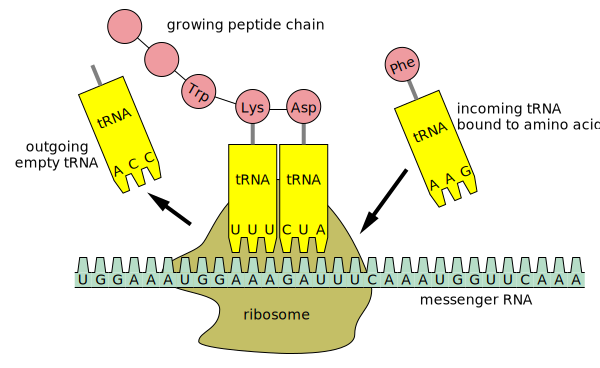
\includegraphics[width=0.49\textwidth]{../frontespizio/tikz/4_lesson/Peptide_syn.png}
    \caption{Transcription of DNA to \emph{mRNA} by \emph{RNA polymerase} on the left. Peptide systesis on the right.}
\end{figure}
This "dogma" is therfore not a real one, as Francis Crick had defined it. Further discoveries have highlighted this possibility of DNA modification by proteins and macromolecules: the study of such effects is called \textbf{epigenetics}, meaning \emph{on top of genetics} from the Greek. Moreover, random point mutation can change either permanently or temporarily the DNA and we have to point out that even multiple clones of the same animal are not completely identical, since they share both the same DNA and also, since the come from a common egg, its cytoplasm. 
We can think also of viruses that modify DNA, by manipulating the specif protein production.   
\marginpar{ \textbf{Exercise 1.}}



\chapter{Brownian motion}
Molecules are immersed in water and they jiggle all the time due to collisions with $H_2 O$ molecules. Even though water molecules (Figure \ref{fig:water}) are smaller than the particles we are here considering, but $10^{12}$ is the number of collisions per seconds (?) estimated to which particles are subjected to. This is responsible for the presence of a random force that make particles move randomically in space, making them describing casual patterns. 
\section{Law of diffusion}
\subsection{Random walk model}
The paths described by particles are continuous and not differentiable, as well as scale invariant: in fact, zooming in a specific pattern, it is possible to ascertain the fractacl geometry of the trajectories described.  

Let's consider a $1-dim$ problem for semplicity, in which, at each time step:
\begin{itemize}
    \item the particle make a jump of length $\Delta L>0$, independent from the previous step, with equal probability to the left or to the right: $P_+=P_-=\frac{1}{2}$;
    \item each time interval is deterministic\footnote{We won't consider the case of random $\Delta t_i$, so dealing with a \emph{continuous random walk model}.}: $\Delta t>0$;
    \item $p_i(N)$ is the probability of finding the particle in position $x_i(N)=i\Delta L$, with $i\in\mathbb{Z}$, aftern $N$ steps, so after a time $t=N\Delta t$. 
\end{itemize}

To formally reproduce a possible trajectory, we will state the \textbf{Langevin equation}, a \emph{stochastic differential equation} (\textbf{SDE}) which uses lagrangian coordinates $\vec{r}(t)$. In eulerian coordinates, instead, $\vec{r}$ is fixed but there is a field $\rho(\vec{r},t)$ that gathers the stochasticity information of the process, so it expresses the probability of finding the particle somewhere. These considerations will lead us to the \emph{partial derivative equation} (deterministic equation) known as the \textbf{Fokker-Planck equation}.

A possible way of formulating $p_i(N)$ is by considering all the paths $M_i(N)$ of $N$ steps ending at position $x_i=i\Delta L$: $p_i(N)=\frac{M_i(N)}{M(N)}$ where $M(N)$ is the total number paths obtainable within $N$ steps. This last variable is easy to compute, since the particle can equally jump to the right or to the left, $M(N)=\underbrace{2\cdot2\cdot2\dots\cdot2}_{\text{$N$-terms}}=2^N$. \\
Defining $N_r$ the number of steps the particle takes to the right and $N_l=N-N_r$ the number of steps it takes to the left, then:
\begin{equation*}
    \begin{split}
        x_i(N) = i\Delta L &= N_r\Delta L+N_l(-\Delta L) \\
        &= (N_r-N_l)\Delta L = (2N_r-N)\Delta L 
    \end{split}
\end{equation*}
From $i=(2N_r-N)\implies N_r = \frac{N+i}{2}$. If we consider exactly $N$ steps, we can have many different patterns, starting at different positions, which stop in $i$: to count them we have to consider all the possible way to group $N$ objects in $N_r$ subgroups, so basically considering a binomial distribution given by:
\[
    M_i(N) = \binom{N}{N_r}=\frac{N!}{(N-N_r)!(N_r)!} = \frac{N!}{(\frac{N-i}{2})!(\frac{N+i}{2})!}
\]
Note that there is no problem in computing this binomial since $N$ and $i$ must have the same parity: if $i$ is odd (even) there is no possible way of reaching position $x_i$ in an even (odd) number of steps $N$. 
In conlusion, the sought probability is 
\begin{equation}
    p_i(N) = 
    \begin{cases}
        \frac{1}{2^N}\:\frac{N!}{(\frac{N+i}{2})!(\frac{N-i}{2})!} & \text{if $i$ and $N$ share the same parity,} \\
        0 & \text{otherwise.}
    \end{cases}
\end{equation}   


In lagrangian coordinates $x(N)$ is the position of the particle after exactly $N$ steps. Then:
\begin{equation}
    \vmedvec{x(N)}=0
    \label{eq:mean_zero}
\end{equation}

since, in this model, the particle has the same probability of going either to the left or to the right. 
Expressing $x(N)=x(N-1)+k(N)$, where $k(N)=\pm \Delta L$, we have that $$\vmedvec{x(N)^2}\myeq{a}\vmedvec{x(N-1)^2}+2\vmedvec{x(N-1)\cdot k(N)}+\vmedvec{k(N)^2}$$ where in $(a)$ we have expanded the square and applied the linearity of the mean value. We observe now that $\vmedvec{x(N-1)\cdot k(N)}=\vmedvec{x(N-1)}\vmedvec{k(N)}$ because steps are independent one from the other. Furthermore, as equation [\ref{eq:mean_zero}], $\vmedvec{x(N-1)}=0$ and also $\vmedvec{k(N)}=0$ from its definition: these relations actually describe the so called \textbf{Markovian process}\cite{Markov}, a stochastic model describing a sequence of possible events where the probability could depend only on the state attained in the previous event - \emph{order 1 Markovian process} for the $x$ variable - or can be completely memoryless - \emph{order 0 Markovian process} for the $k$ variable - so where there is no dependency on previous steps.

In conclusion: $\vmedvec{x(N)^2}=\vmedvec{x(N-1)^2}+\Delta L^2$. Considering $N=2$, we have that $\vmedvec{x(2)^2}=\underbrace{\vmedvec{x(1)^2}}_{=\Delta L^2}+\Delta L^2=2\Delta L^2$. By induction we can finally find the \textbf{law of diffusion}:
\begin{equation}
    \mathcolorbox{yellow}{\vmedvec{x(N)^2}}=N\Delta L^2=\frac{t}{\Delta t}\:\Delta L^2=t\:\frac{2\Delta L^2}{2\Delta t}=\mathcolorbox{yellow}{2Dt}
    \label{eq:diffusion}
\end{equation} 
$D=\frac{\Delta L^2}{2\Delta t}$ is the diffusion coefficient which, as a \emph{transport coefficient} as dimensions $[D]=\frac{\mathbb{L}^2}{\mathbb{T}}$.\\
In $3-dim$ this can be easily extended to: 
\begin{equation}
    \vmedvec{\vec{r}^{\:2}}=\vmedvec{x(t)^2}+\vmedvec{y(t)^2}+\vmedvec{z(t)^2}=6Dt
    \label{eq:diffusion_3D}
\end{equation}
    \subsection{Diffusion processes in biological organism}
Now that we have uncovered the main law of diffusion, seeing as the variance of this kind of processes grows linearly in time, we ask ourselves: \emph{is diffusion a good mechanism for transport?}\\
To answer this question, suppose we have two spherical - for simplicty - cells of radius $R=1\mu m$ (size of an \emph{E. Coli} approximately) and $R=10\mu m$ (size of an \emph{eukaryotic} cell approximately) respectively. In the center of these cells there is a specific biological compound such as a glucouse molecule or a globular protein. They have diffusion coefficients $D_{C_6H_{12}O_6}\simeq10^{-9}m^2/s=1\mu m^2/ms$ and $D_{protein}\simeq10^{-2}\mu m^2/ms$ respectively\footnote{Notice how the diffusion coefficient is smaller for bigger cells: the bigger the cell the less molecules tend to diffuse}. The time $\tau$ needed for the molecule to diffuse outside the cell, so to walk a distance $R$, is given by equation [\ref{eq:diffusion_3D}]: $R^2=6D\tau\implies \tau=\frac{R^2}{6D}$.

\begin{table}[h!]
    \centering
    \caption{\label{diffusion time} Diffusion time.}
    \resizebox{\textwidth}{!}{%
    \begin{tabular}{l|l|l}
     & Glucose molecule - $C_6 H_{12} O_6$ & Globular protein \\ \hline
    \emph{E. coli} & $\tau\simeq0.2\:ms$ & $\tau\simeq20\:ms$ \\
    \emph{Eukaryotic cell} & $\tau\simeq20\:ms$ & $\tau\simeq2\:s$
    \end{tabular}%
    }
\end{table}

As shown in Table [\ref{diffusion time}], diffusion is an ideal process for small enough organism, in the case there is the need of transport of tiny molecules. Otherwise, diffusion is not efficient: think, just for example, that brain signals travels on average at $\tau\simeq2\:ms$: this means that there exist other forms of trasport, of \emph{active transport} specifically, in which cells spend some energy - ATP molecules - to carry out things in specific directions. Diffusion represents a \emph{passive transport} mechanism, perfect for spreading in all directions, mostly because it is energy free, since it is the direct consequence of thermal activity of the environment in which cells are plunged.

\end{document}